\documentclass[12pt,a4paper]{ctexart}
\usepackage[a4paper,margin=2.2cm]{geometry}
\usepackage{graphicx}
\usepackage{booktabs}
\usepackage{float}
\usepackage{enumitem}
\usepackage{array}
\usepackage{longtable}
\usepackage{amsmath}
\usepackage{caption}
\captionsetup{font=small}

\begin{document}

\begin{center}
{\LARGE \textbf{上机实验报告——特征选择数据集划分与线性回归}}\\[1em]
学号：\underline{\hspace{4cm}} \hspace{2cm} 姓名：\underline{\hspace{3cm}}
\end{center}

\vspace{1em}

\section*{一、实验目的}
\begin{enumerate}[label=（\arabic*）]
\item 掌握特征选择的基本思路与实现方法，筛选有效特征。
\item 学会将数据集正确划分为训练集与测试集。
\item 掌握线性回归模型的构建、训练、预测与评价。
\item 巩固数据预处理流程。
\end{enumerate}

\section*{二、实验环境}
\begin{enumerate}[label=（\arabic*）]
\item 编程语言：Python
\item 核心库：
\end{enumerate}

\noindent pandas、numpy：数据读取与数值计算\\
\noindent sklearn：数据集划分、线性回归、评估指标\\
\noindent matplotlib/seaborn：可视化

\section*{三、实验数据介绍（对使用数据集作介绍）}
本实验使用的数据由 \texttt{get\_data.py} 抓取并导出，数据文件为 \texttt{code/沪深300\_最近三年.csv}。数据内容为沪深300指数近三年的日线交易数据，共 725 条样本、7 个原始字段，分别为：日期、收盘、开盘、高、低、交易量、涨跌幅。

其中，收盘价作为本次线性回归任务的目标变量；开盘价、最高价、最低价和交易量作为候选输入特征；涨跌幅虽然能反映价格变化，但它是根据收盘价计算得到的，因此在特征选择时需要考虑目标泄漏问题。数据总体时间跨度从 2023 年 3 月 20 日到 2026 年 3 月 18 日，具有明显的时间顺序特征。

\begin{table}[H]
\centering
\begin{tabular}{>{\raggedright\arraybackslash}p{3cm} >{\raggedright\arraybackslash}p{9.5cm}}
\toprule
字段 & 含义 \\
\midrule
日期 & 交易日期 \\
收盘 & 当日收盘价，作为目标变量 \\
开盘 & 当日开盘价 \\
高 & 当日最高价 \\
低 & 当日最低价 \\
交易量 & 当日交易量，原始格式带有 K \\
涨跌幅 & 相对前一交易日收盘价的涨跌百分比 \\
\bottomrule
\end{tabular}
\end{table}

\section*{四、实验内容与步骤}

\subsection*{1. 数据加载与预处理（读取数据集,处理缺失值、异常值、重复行,分离特征矩阵和目标变量）}
首先读取 \texttt{CSV} 数据文件，并将日期字段转换为日期类型。随后将交易量中的 \texttt{K} 去除并转换为数值型，将涨跌幅中的百分号去除并转换为数值型。检查发现数据集中仅有 1 个缺失值，位于涨跌幅字段，因此采用中位数进行填充；重复行数量为 0，因此无需删除样本。

在异常值处理部分，采用 IQR 方法识别异常值，并使用截尾（clip）方式减弱极端值的影响。识别结果为：收盘 6 个、开盘 3 个、最高价 1 个、最低价 2 个、交易量 24 个、涨跌幅 34 个。完成清洗后，进一步提取年份、月份、日和星期等日期衍生特征。最后将特征矩阵与目标变量分离，其中目标变量为收盘价。

\begin{figure}[H]
\centering
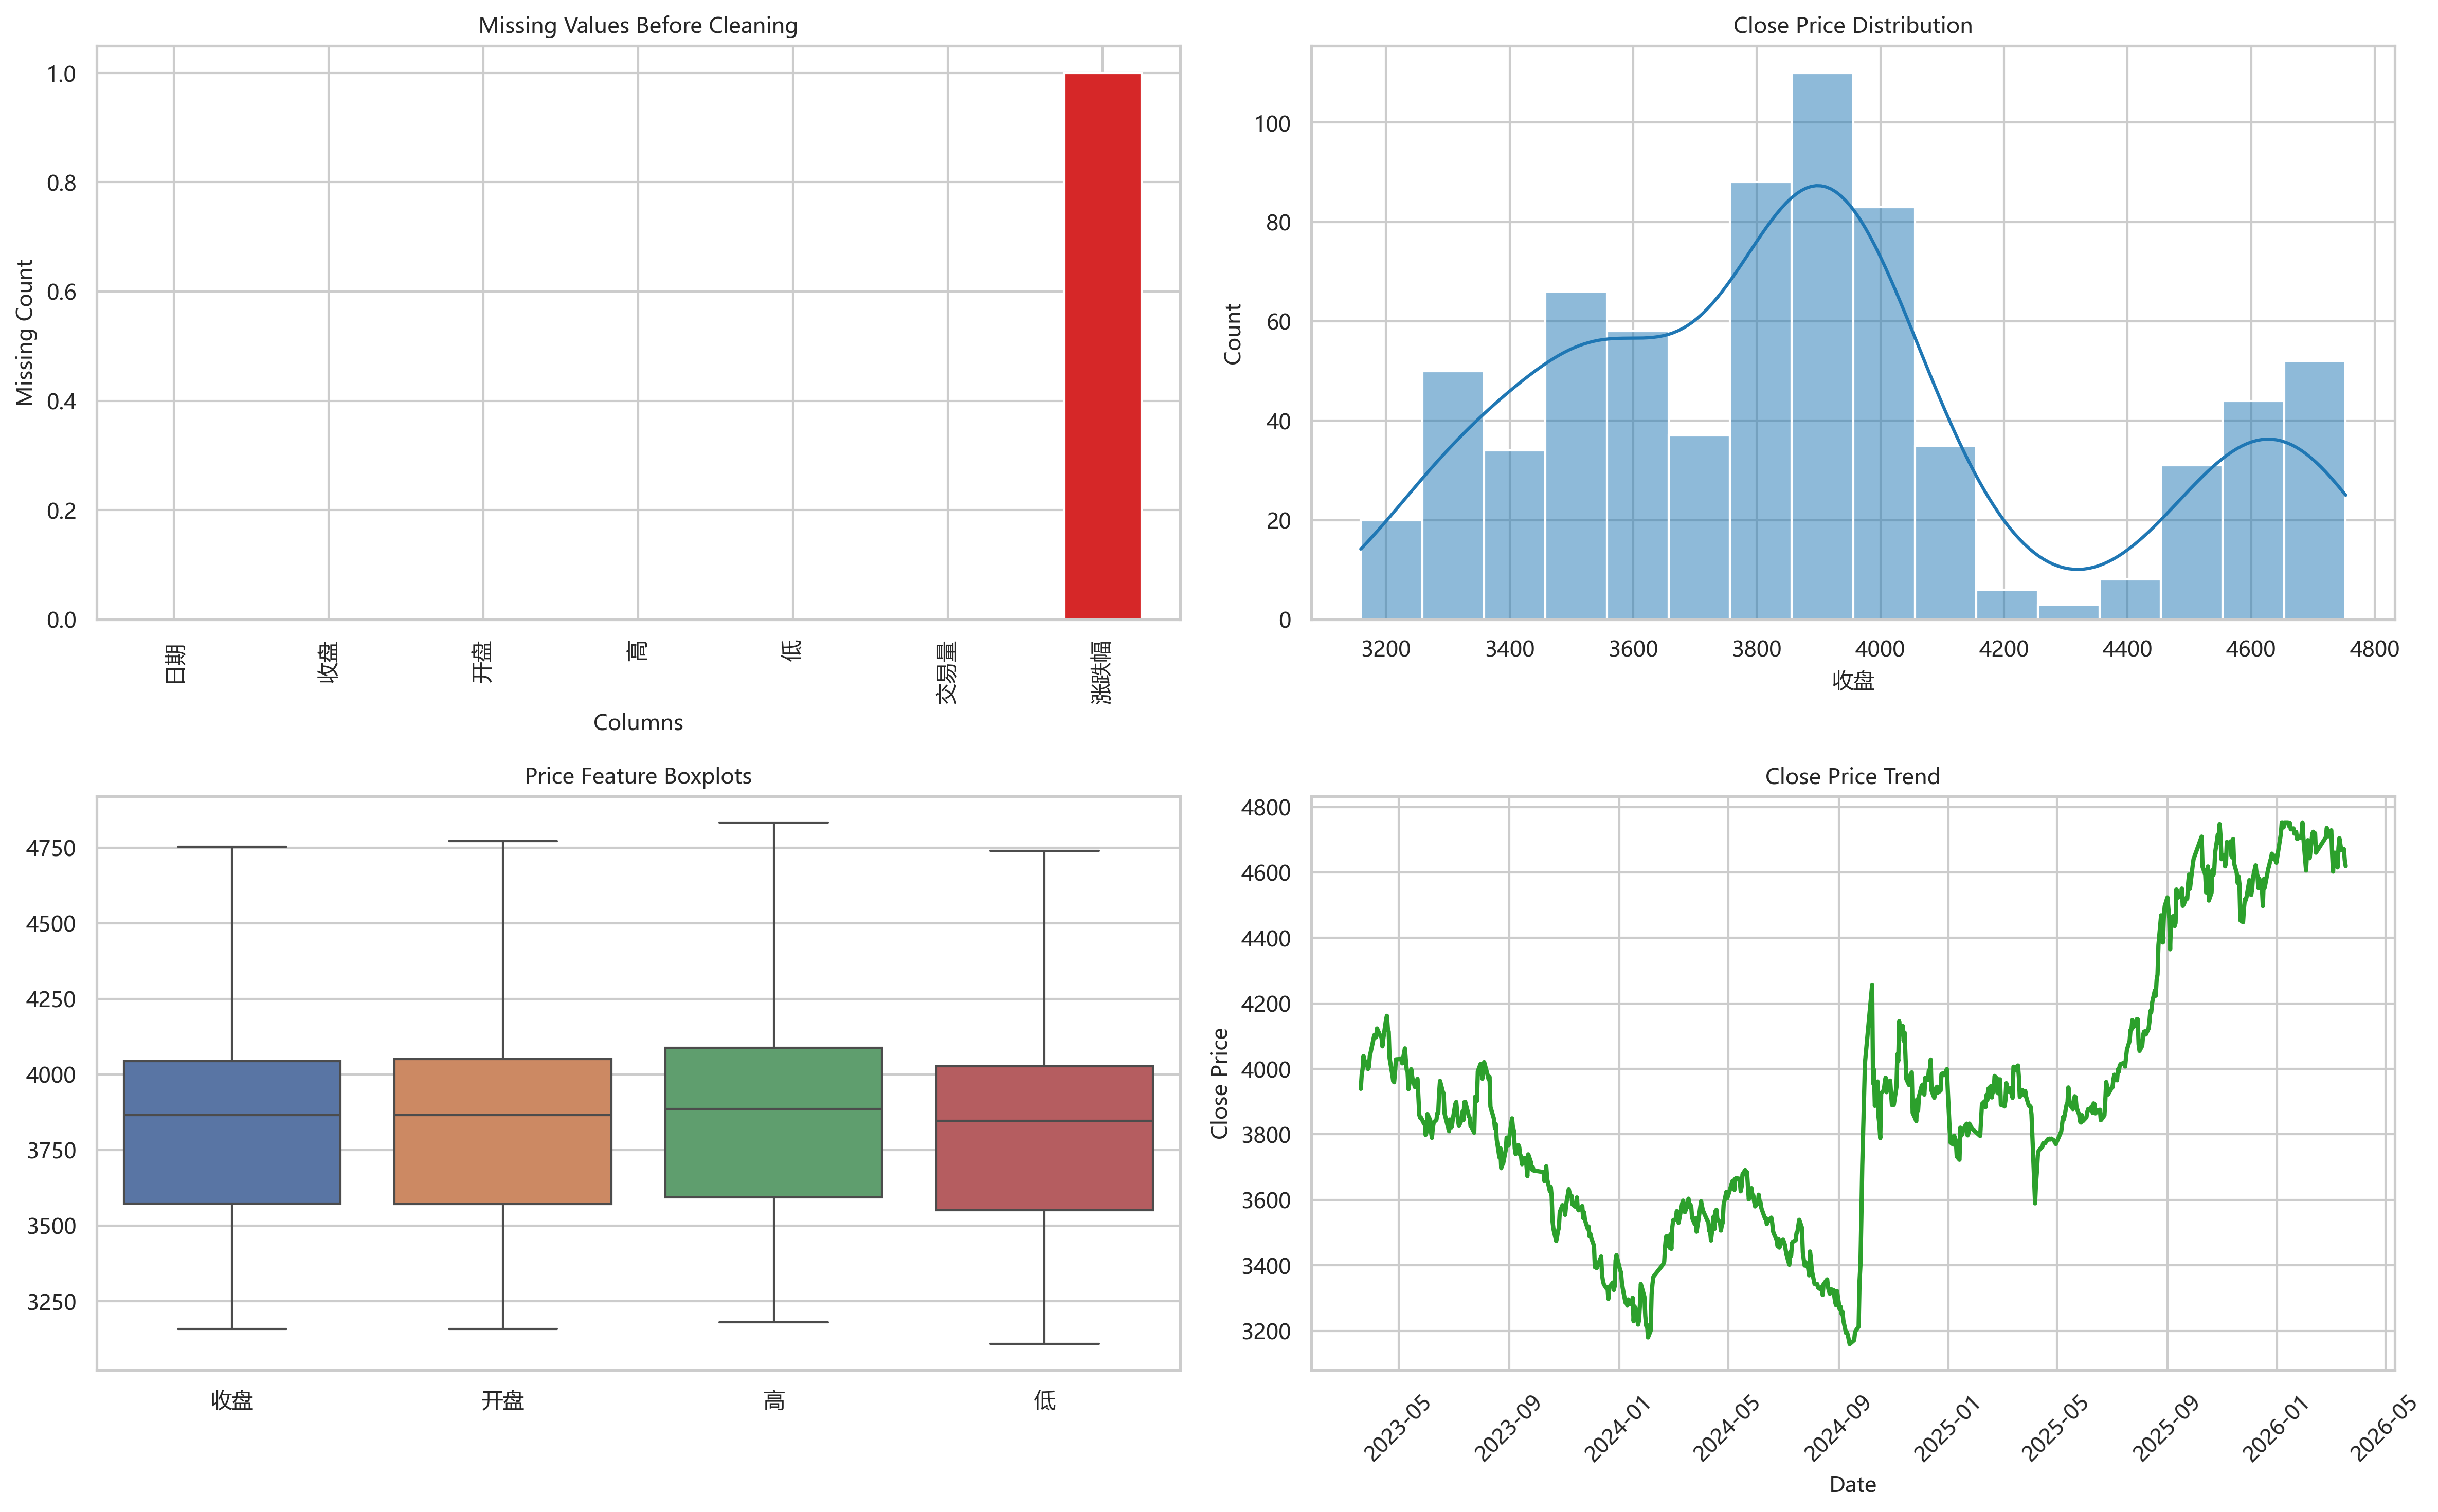
\includegraphics[width=0.92\textwidth]{result/fig1_preprocess_overview.png}
\caption{数据预处理阶段的缺失值统计、收盘价分布、箱线图与走势}
\end{figure}

\begin{figure}[H]
\centering
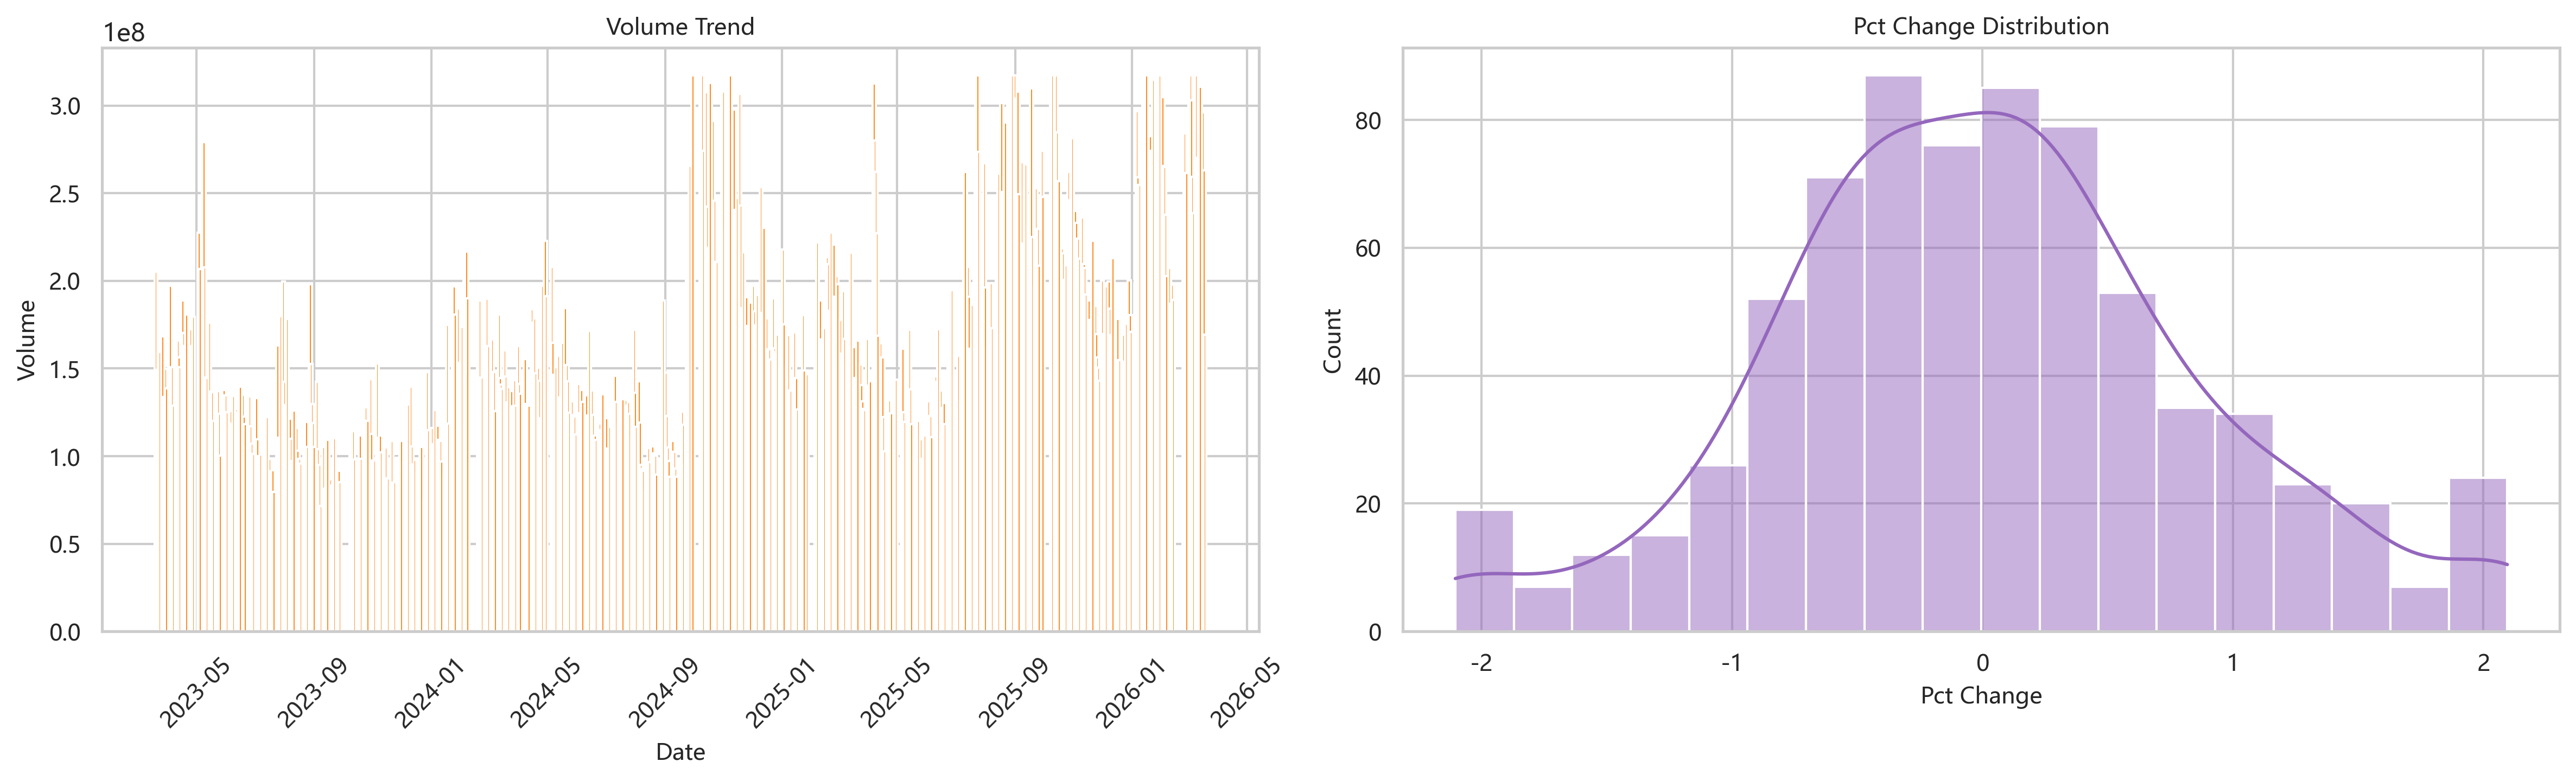
\includegraphics[width=0.88\textwidth]{result/fig2_volume_pct.png}
\caption{交易量趋势与涨跌幅分布}
\end{figure}

\subsection*{2.特征选择（包含：计算特征间相关系数，剔除高度相关冗余特征；剔除单一取值占比过高的无效特征；保留与目标变量相关性较强、有实际意义的特征）}
先计算候选特征之间及其与目标变量之间的相关系数，并绘制相关性热力图。结果表明，开盘价、最高价、最低价与收盘价之间都具有极强相关性，但三者之间彼此也高度相关，属于典型的冗余特征。

接着按照如下规则进行筛选：
\begin{enumerate}[label=（\arabic*）]
\item 若两个特征间相关系数大于 0.95，则保留与目标变量相关性更强的特征；
\item 若单一取值占比过高，则视为无效特征剔除；
\item 若特征与目标变量相关性较弱，则剔除；
\item 若特征由目标变量直接推导得到，则剔除以避免目标泄漏。
\end{enumerate}

根据筛选结果：
\begin{itemize}[leftmargin=2em]
\item 开盘价、最低价与最高价高度相关，最终保留“最高价”，剔除“开盘价”和“最低价”；
\item 涨跌幅由收盘价推导得到，存在目标泄漏风险，因此剔除；
\item 月份、日、星期与目标变量的相关性较弱，因此剔除；
\item 最终保留的特征为：最高价、交易量、年份。
\end{itemize}

\begin{figure}[H]
\centering
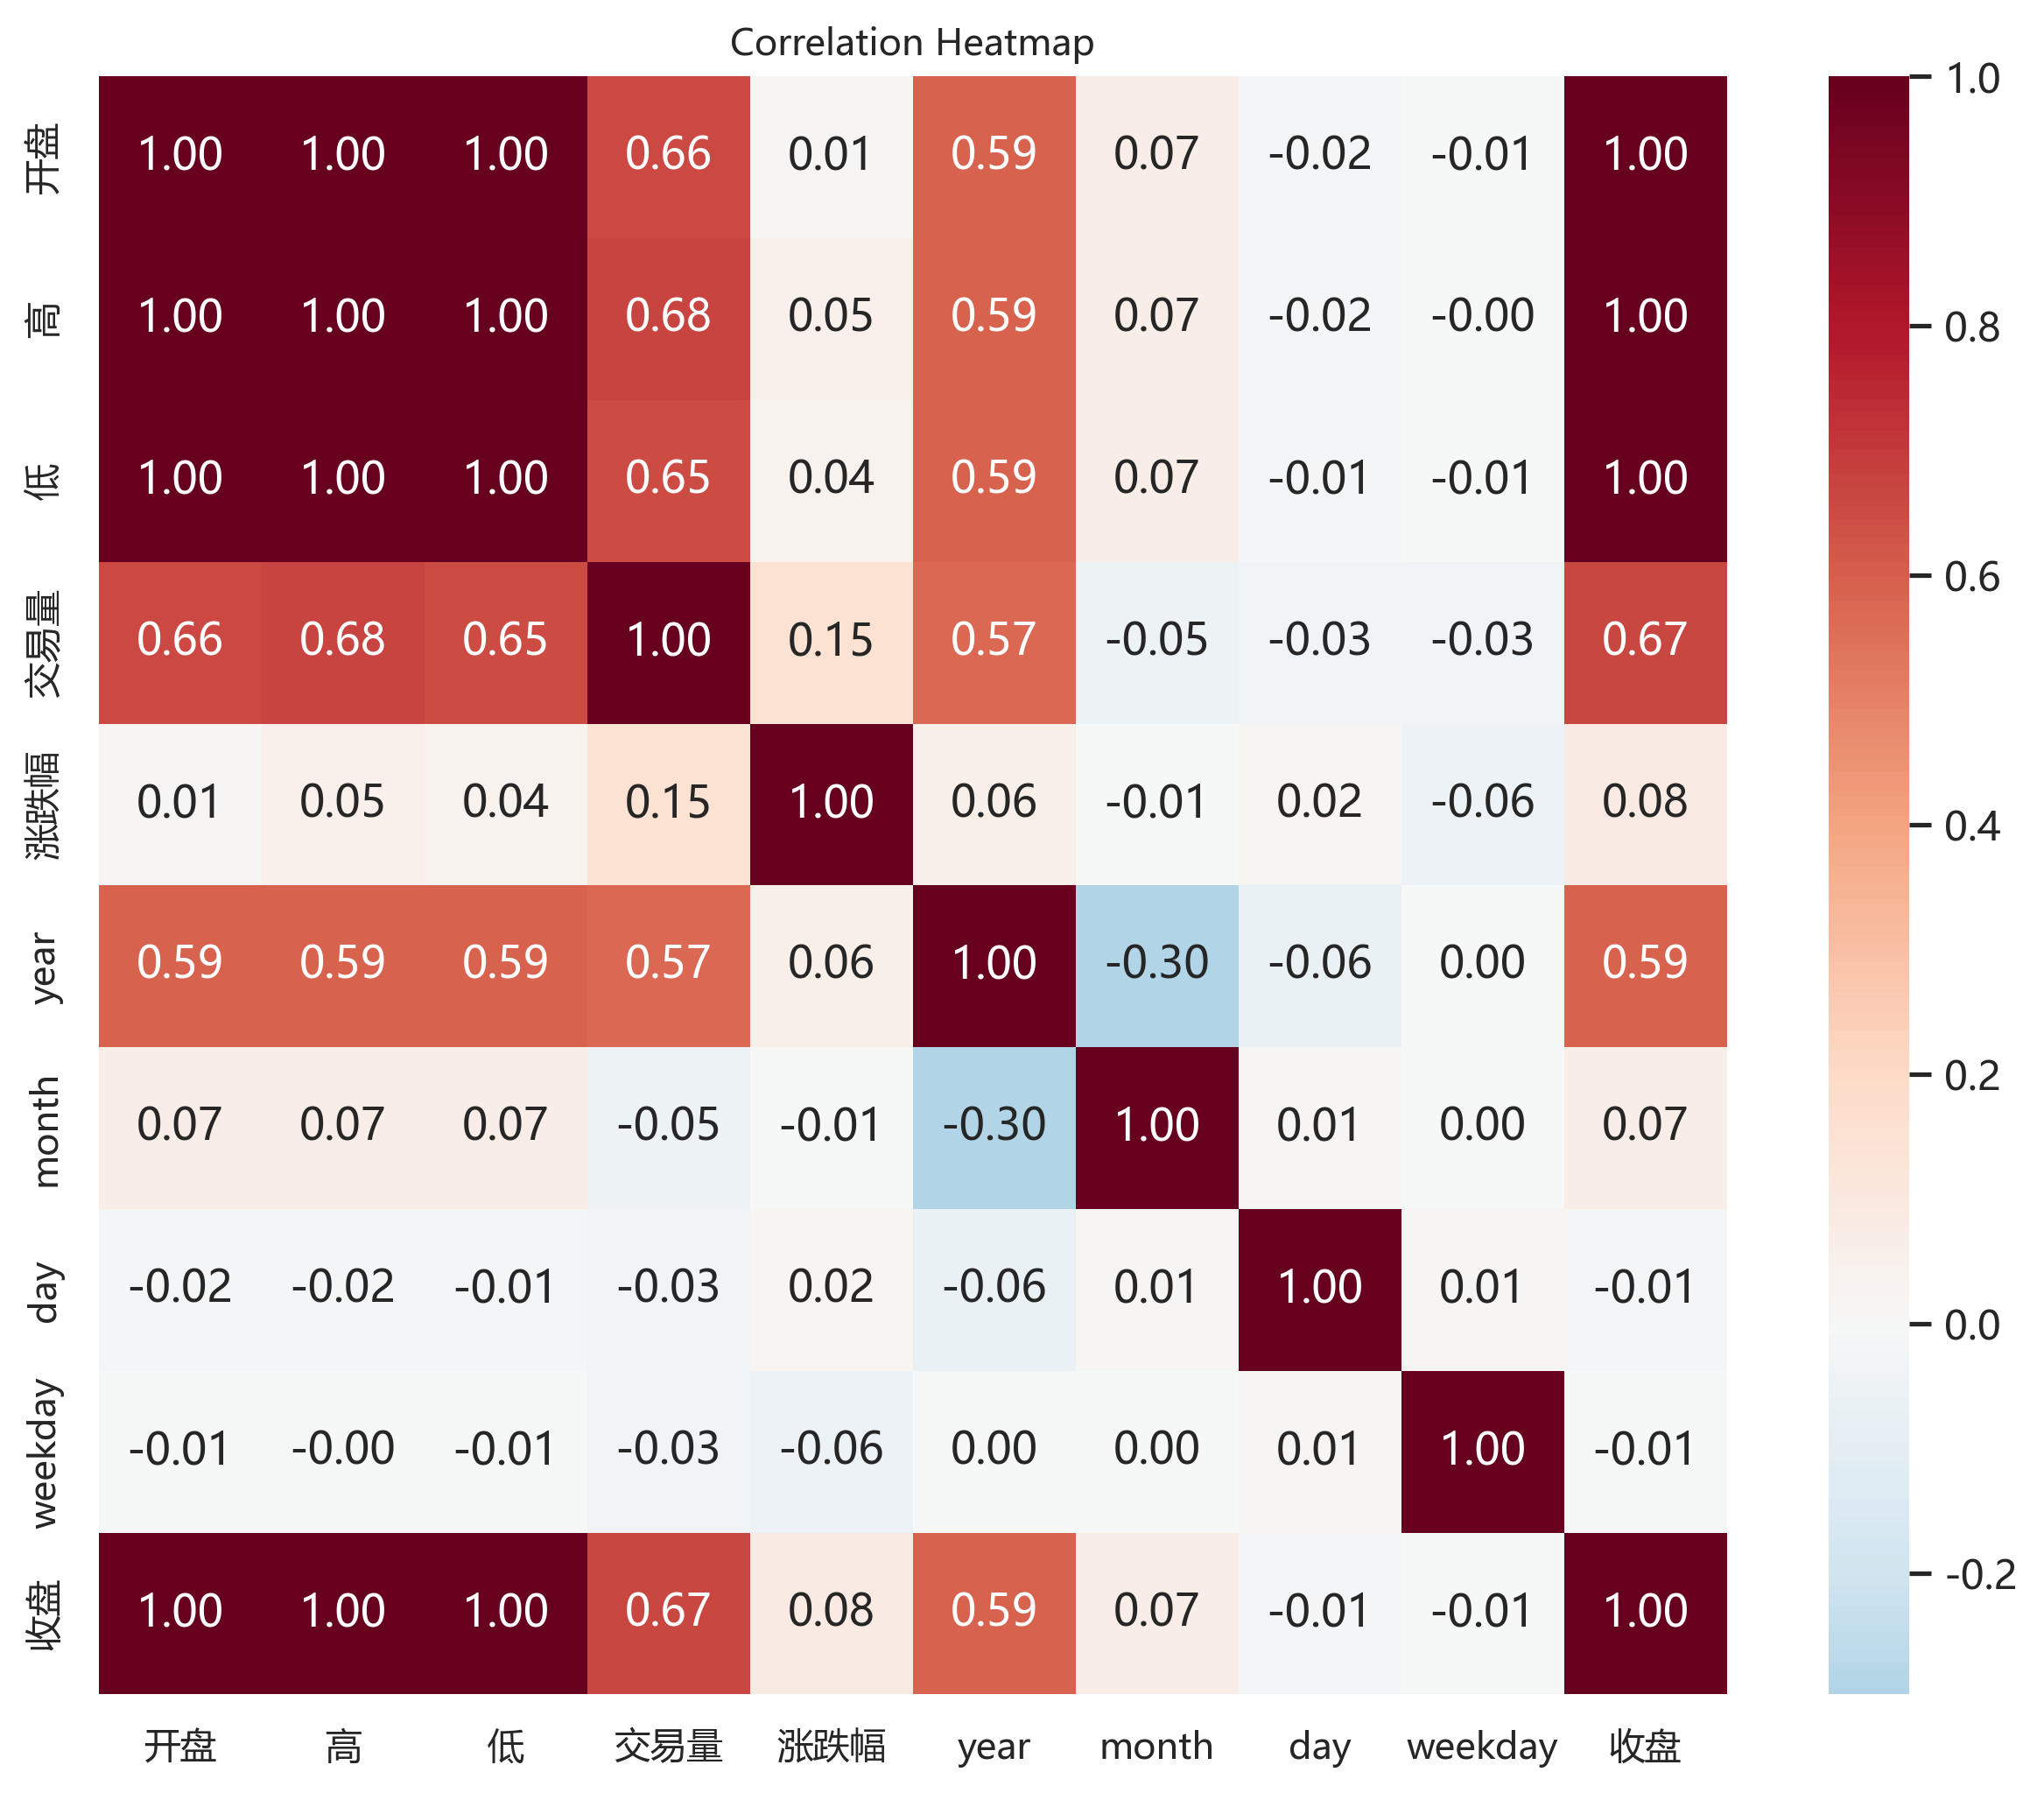
\includegraphics[width=0.82\textwidth]{result/fig3_correlation_heatmap.png}
\caption{候选特征与目标变量的相关性热力图}
\end{figure}

\begin{figure}[H]
\centering
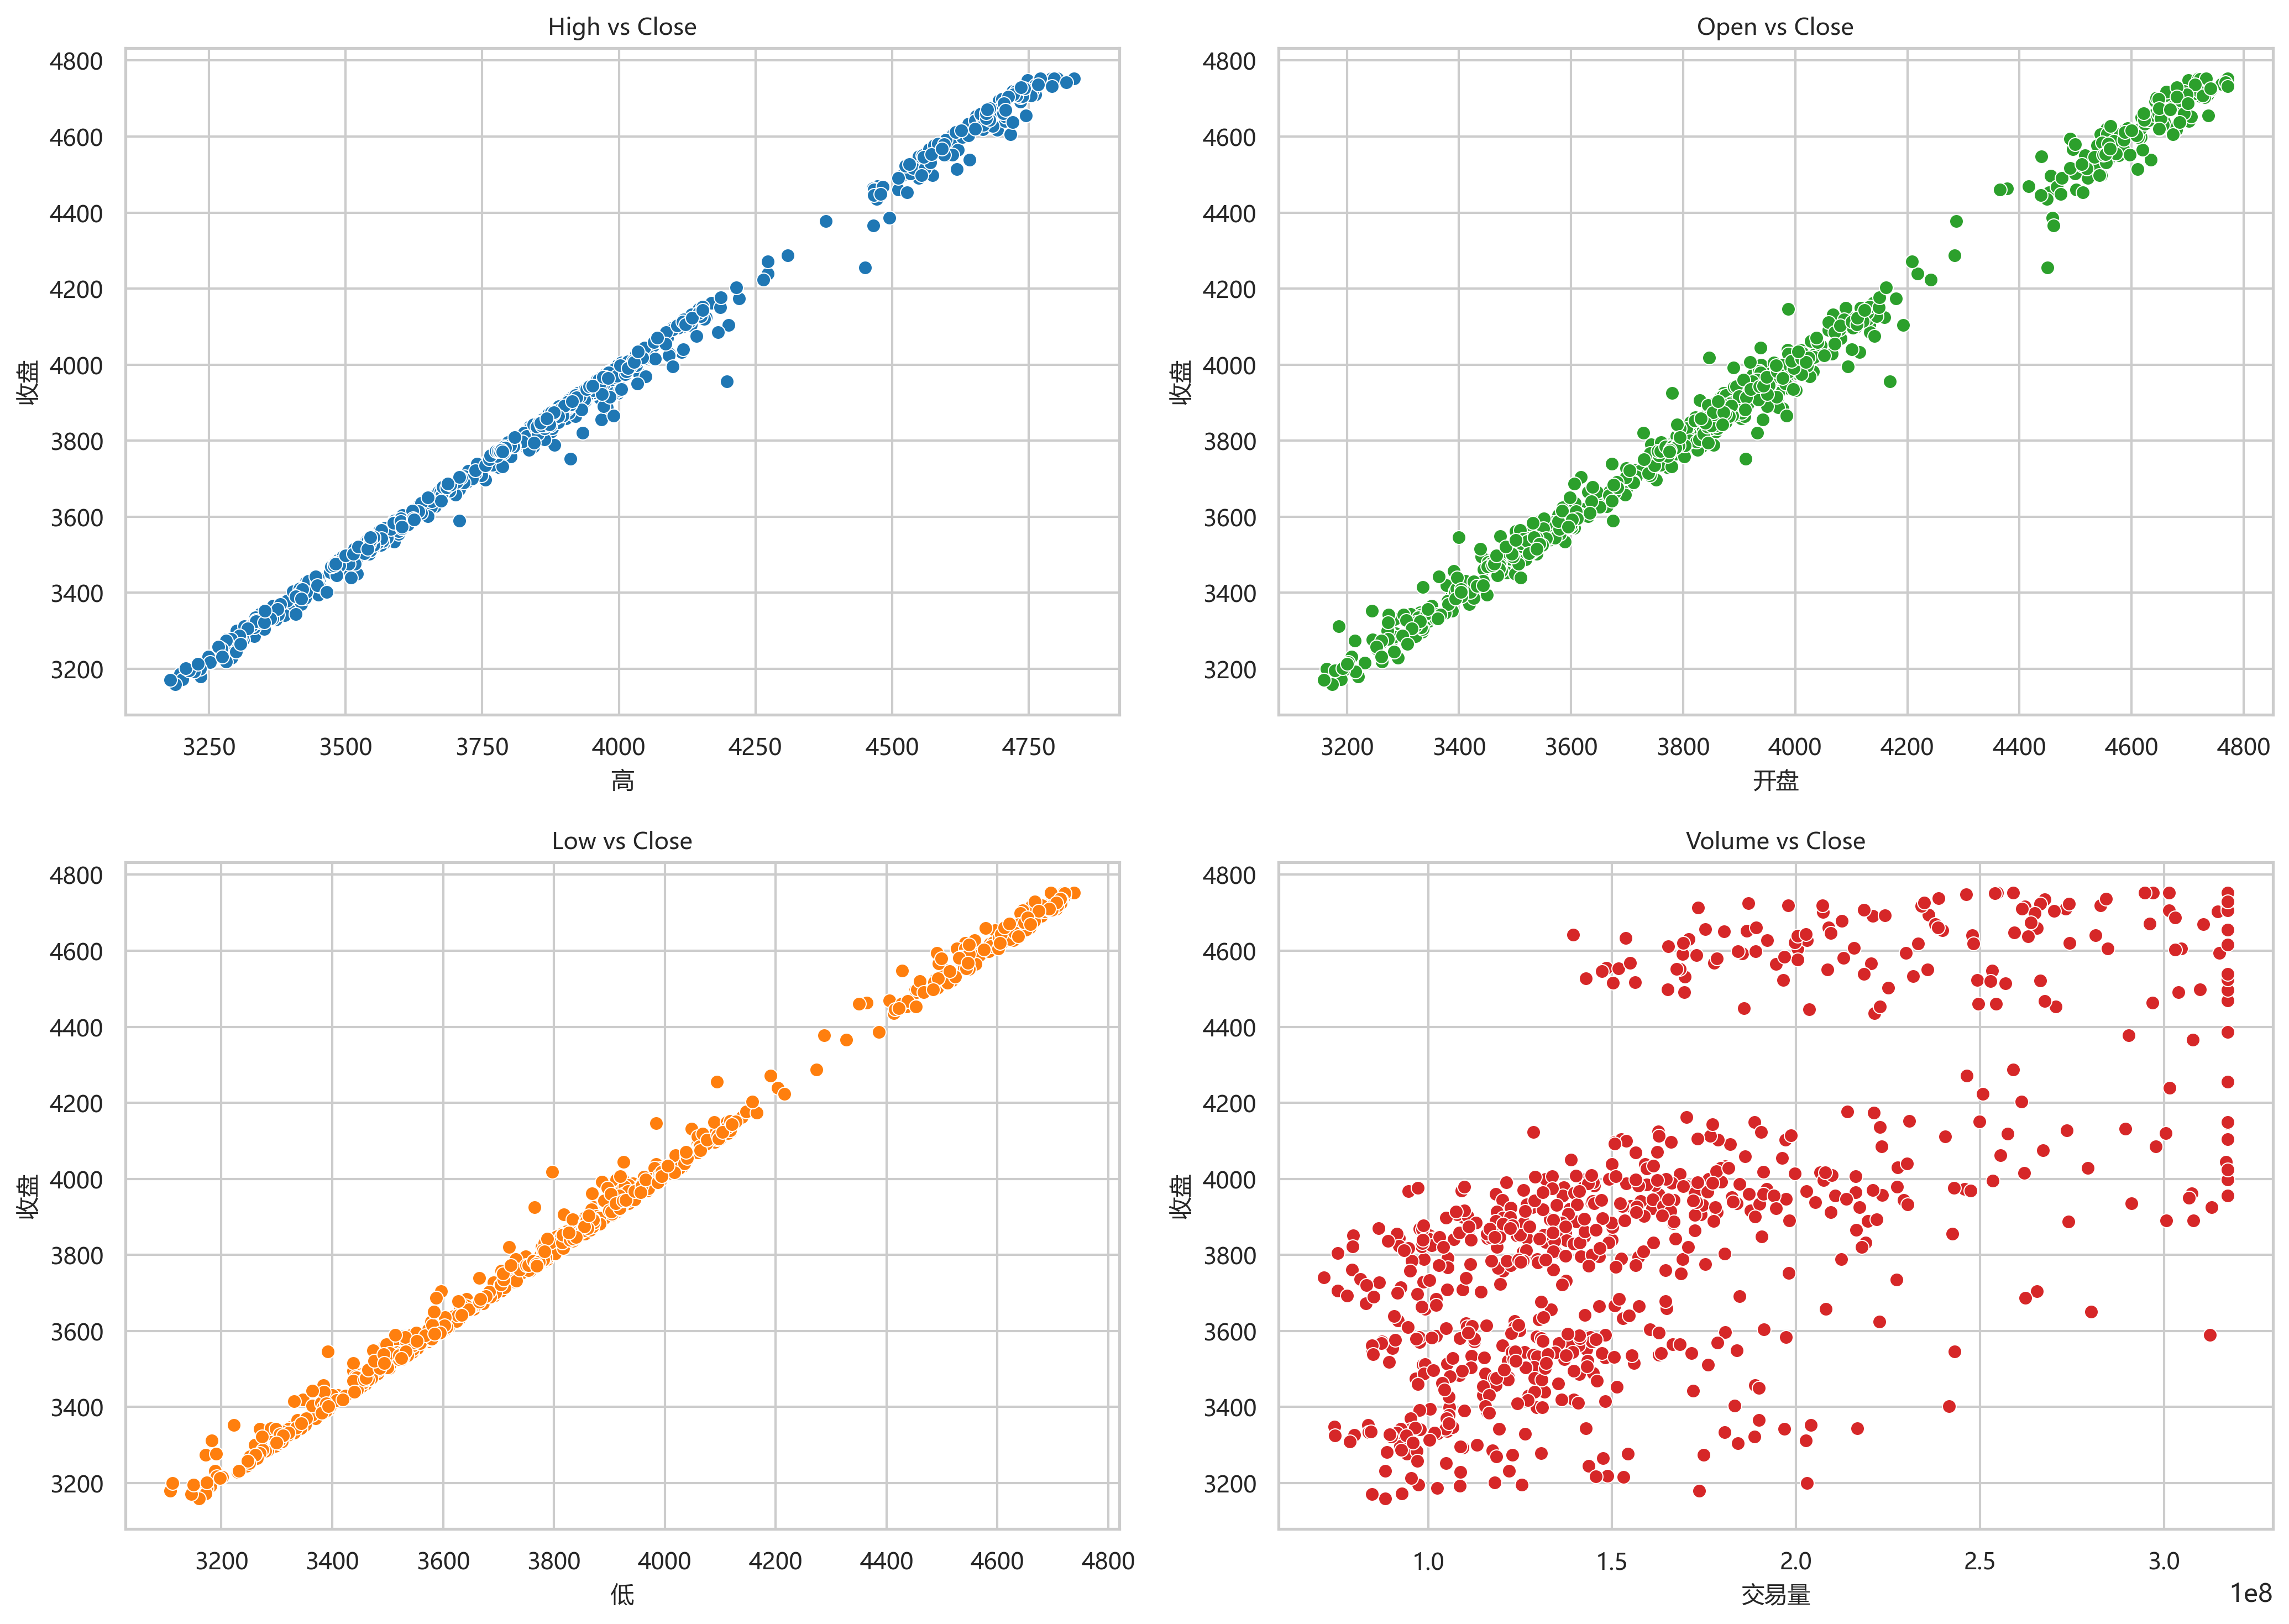
\includegraphics[width=0.92\textwidth]{result/fig4_feature_scatter.png}
\caption{主要候选特征与收盘价的散点关系}
\end{figure}

\subsection*{3. 数据集划分（包含：将数据划分为训练集与测试集，常用比例，训练集 70\%—80\%，测试集 20\%—30\%）}
考虑到本实验数据带有明显时间顺序，如果采用随机打乱划分，会破坏真实的时序结构，因此本实验按照时间先后顺序划分数据集。前 80\% 的样本作为训练集，后 20\% 的样本作为测试集，符合常见的训练集 70\%—80\%、测试集 20\%—30\% 的划分原则。

本次划分结果如下：
\begin{itemize}[leftmargin=2em]
\item 训练集样本数：580
\item 测试集样本数：145
\item 训练集时间范围：2023-03-20 至 2025-08-07
\item 测试集时间范围：2025-08-08 至 2026-03-18
\end{itemize}

\subsection*{4. 构建与训练线性回归模型}
在特征筛选完成后，以“最高价、交易量、年份”为输入特征，以“收盘价”为输出变量，构建多元线性回归模型。模型形式如下：
\[
y=\beta_0+\beta_1x_1+\beta_2x_2+\beta_3x_3
\]
其中，$y$ 表示收盘价，$x_1$、$x_2$、$x_3$ 分别表示最高价、交易量和年份。

模型训练完成后得到的主要参数如下：
\begin{itemize}[leftmargin=2em]
\item 截距：$-8848.0062$
\item 最高价系数：$1.0007$
\item 交易量系数：$-1.7169\times10^{-7}$
\item 年份系数：$4.3716$
\end{itemize}

从系数大小可以看出，最高价是解释收盘价最重要的变量，交易量的影响相对较弱，但仍保留一定辅助解释作用。

\begin{figure}[H]
\centering
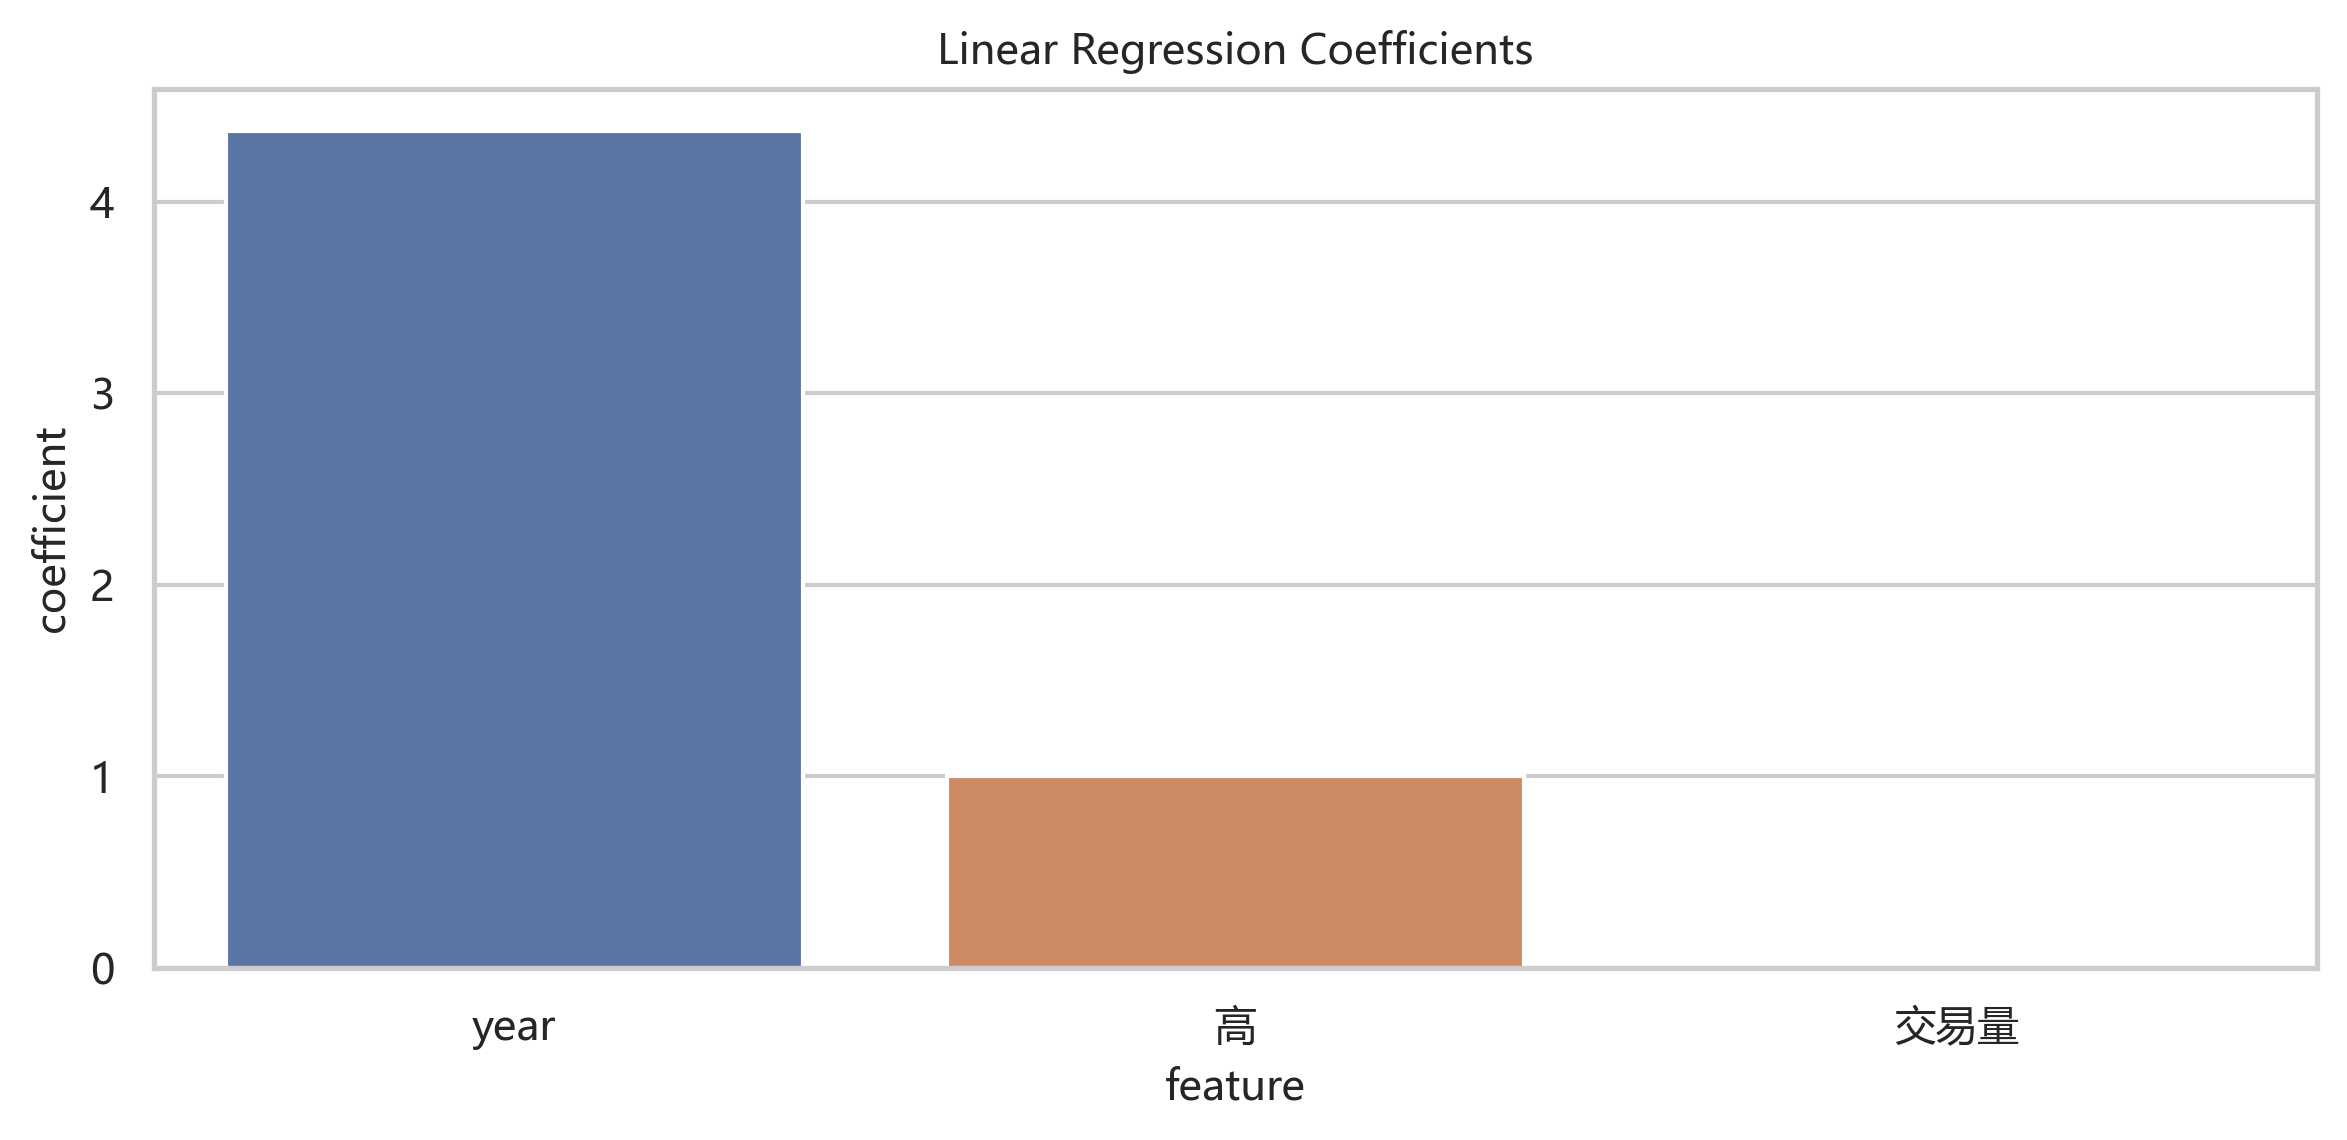
\includegraphics[width=0.68\textwidth]{result/fig5_model_coefficients.png}
\caption{线性回归模型系数图}
\end{figure}

\subsection*{5. 模型预测与评估（用训练好的模型对测试集进行预测，可使用决定系数R²评估模型效果，R² 越接近 1 表示拟合越好）}
使用训练好的线性回归模型对测试集进行预测，并采用训练集 $R^2$、测试集 $R^2$、平均绝对误差 MAE 和均方根误差 RMSE 对模型进行评价。$R^2$ 越接近 1，说明模型拟合效果越好。

本实验得到的评价结果如下：
\begin{table}[H]
\centering
\begin{tabular}{cc}
\toprule
指标 & 数值 \\
\midrule
训练集 $R^2$ & 0.9919 \\
测试集 $R^2$ & 0.9700 \\
MAE & 19.4588 \\
RMSE & 24.3403 \\
\bottomrule
\end{tabular}
\end{table}

从结果来看，测试集上的 $R^2$ 已经接近 1，说明模型对收盘价具有较好的拟合能力。

\begin{figure}[H]
\centering
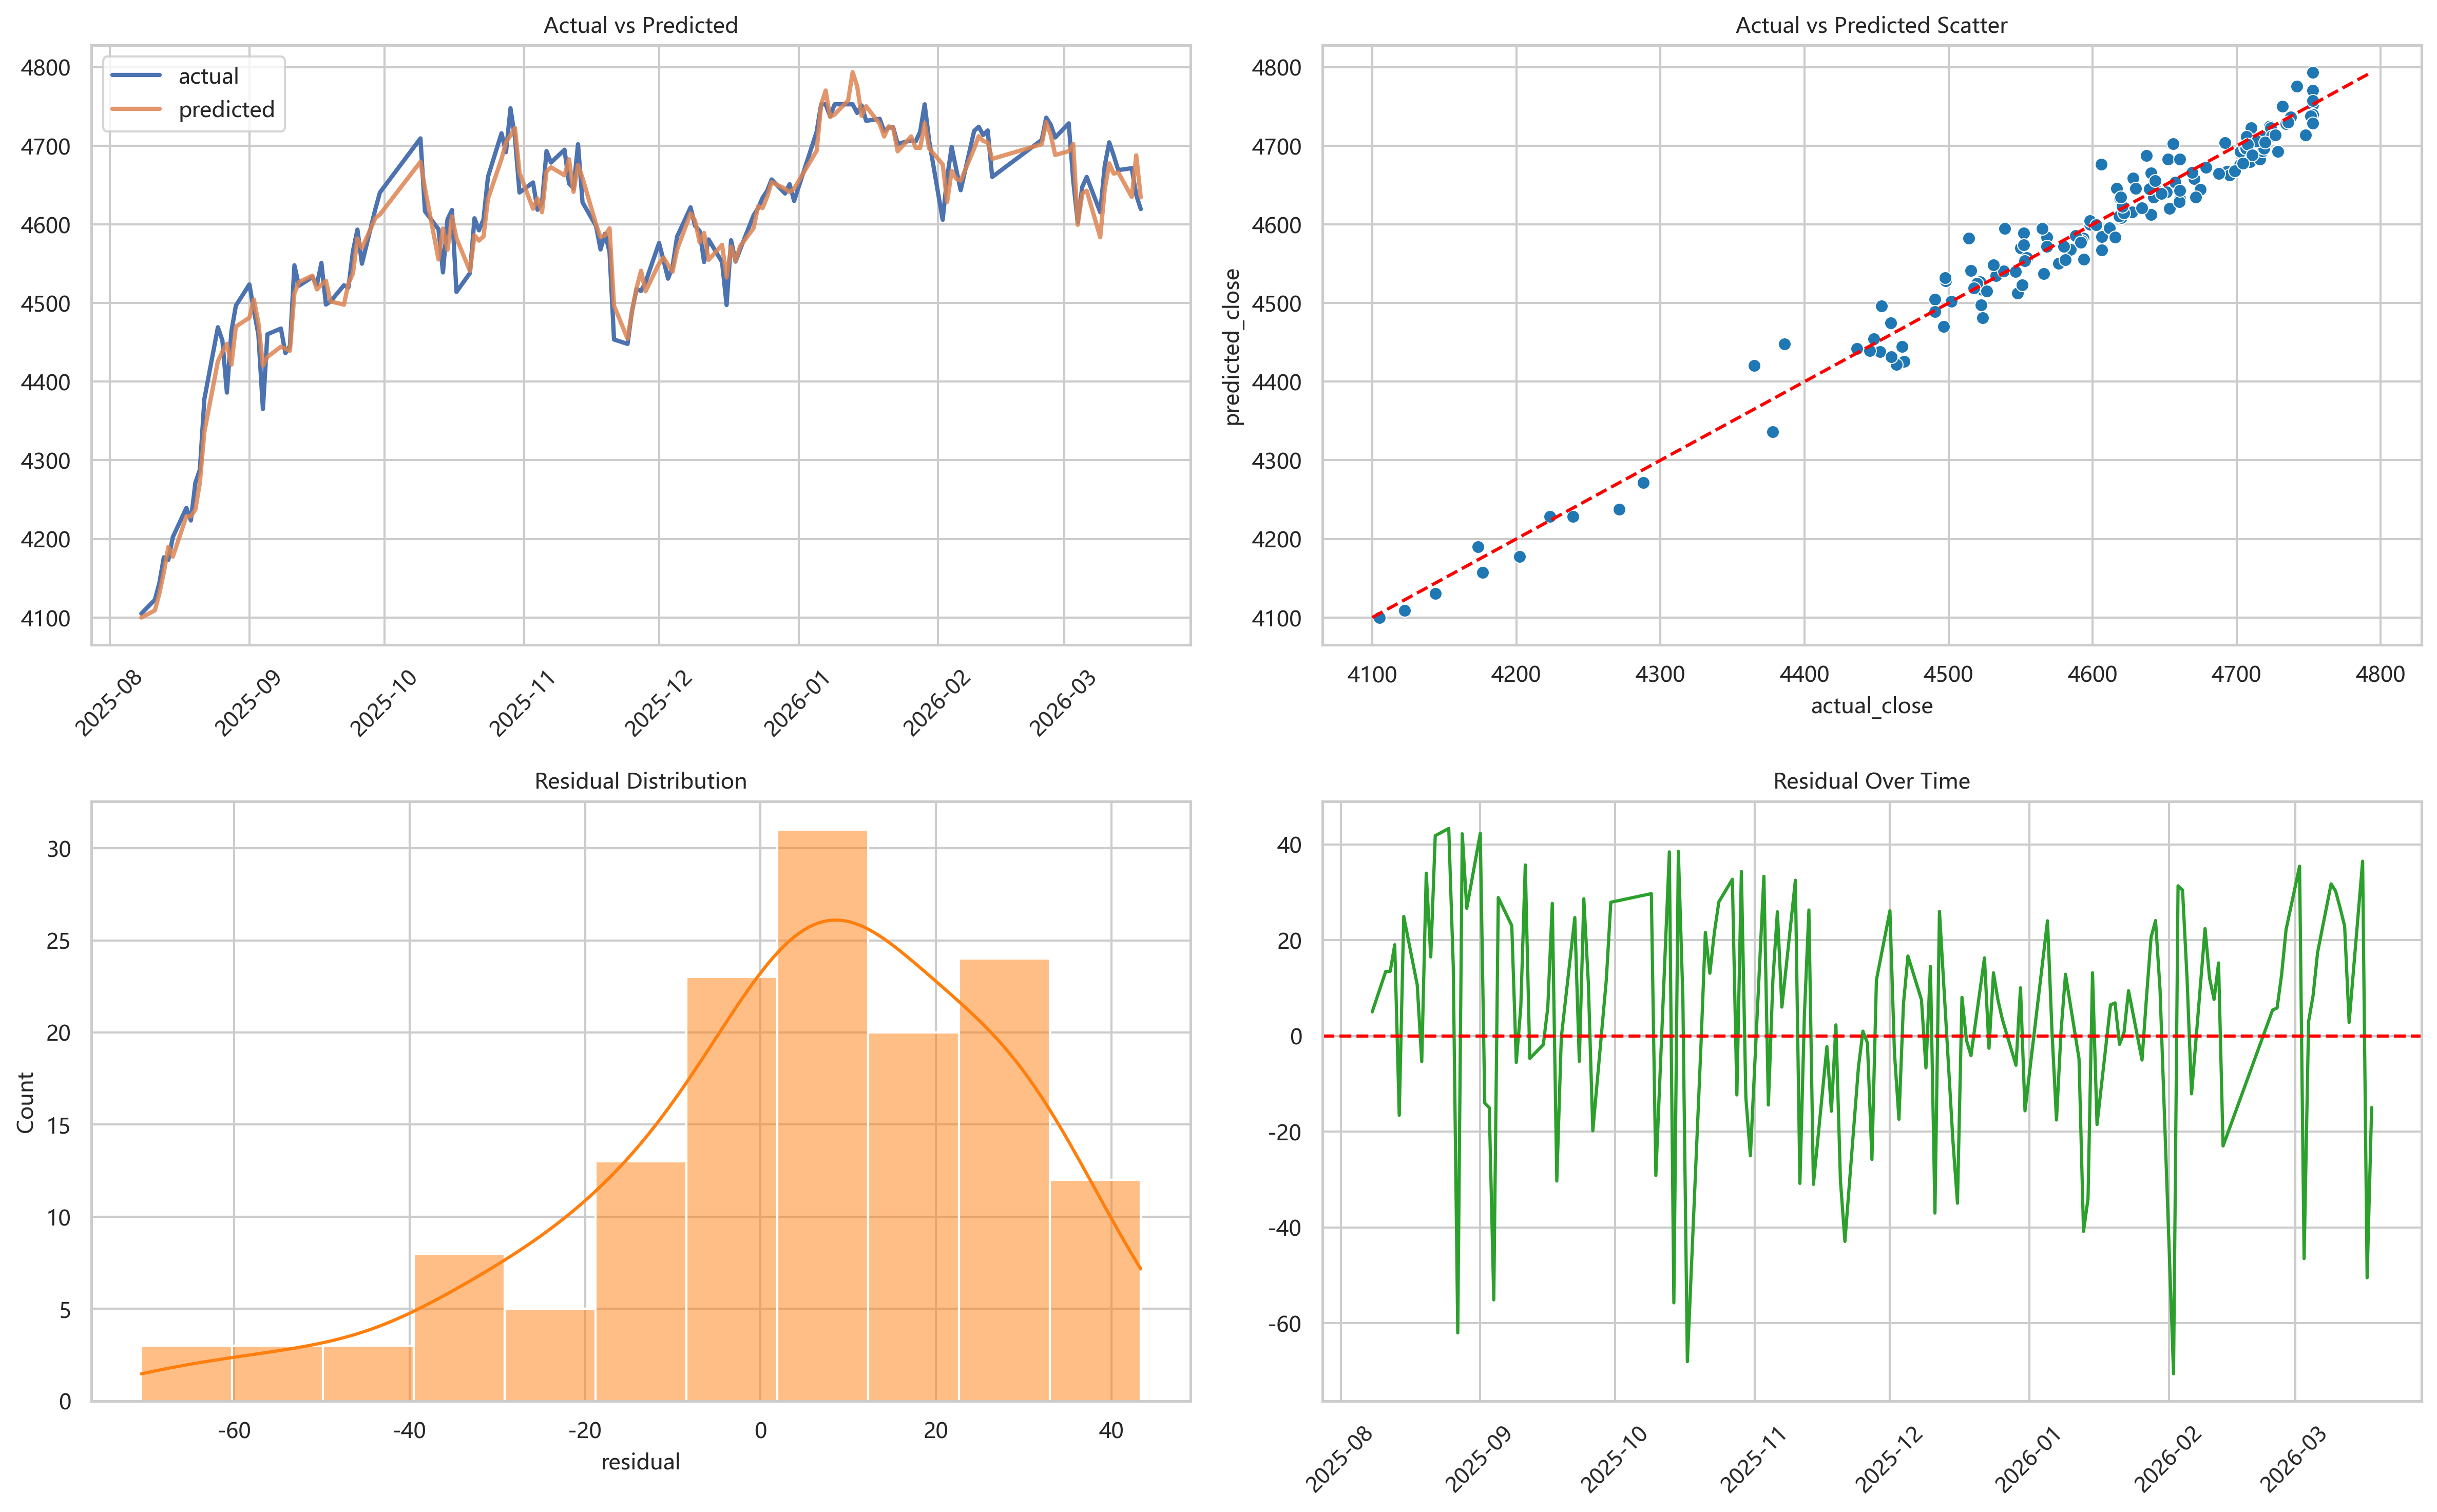
\includegraphics[width=0.92\textwidth]{result/fig6_prediction_residuals.png}
\caption{测试集真实值、预测值及残差分析}
\end{figure}

\subsection*{6.其他，可选做}
除完成基本要求外，本实验还补充了多种可视化分析，包括缺失值图、价格分布图、箱线图、趋势图、相关性热力图、散点图、模型系数图和残差分析图。这些图形可以更直观地展示数据特征与模型效果，也便于在实验报告中进行分析说明。

\section*{五、实验结果与分析（保留的特征列表及选择理由，描述训练集和测试集样本数量，训练集与测试集的 R²分数，对模型效果进行评价）}
本实验最终保留的特征列表为：\textbf{最高价、交易量、年份}。

保留理由如下：
\begin{enumerate}[label=（\arabic*）]
\item 最高价与收盘价绝对相关系数最高，且与收盘价具有较强线性关系；
\item 交易量能够反映市场活跃度，虽然相关性弱于价格类变量，但仍具有实际意义；
\item 年份能够刻画不同年度市场整体水平差异，因此保留；
\item 开盘价和最低价由于与最高价高度相关，属于冗余特征，因此剔除；
\item 涨跌幅由收盘价直接推导得到，存在目标泄漏，因此剔除；
\item 月份、日、星期与目标变量相关性较弱，因此剔除。
\end{enumerate}

训练集和测试集样本数量分别为 580 和 145。模型在训练集上的 $R^2$ 为 0.9919，在测试集上的 $R^2$ 为 0.9700，说明模型在训练集和测试集上都具有较强的拟合能力，且泛化效果较好。结合 MAE 和 RMSE 指标可知，预测误差整体较小，模型性能较稳定。

需要说明的是，本实验数据本质上属于时间序列数据，而线性回归模型属于基础监督学习模型，虽然可以完成课程作业要求，但在真实金融预测场景下仍可进一步尝试更复杂的时序模型。

\section*{六、实验总结}
通过本次实验，完成了从数据读取、数据清洗、特征选择、数据集划分到线性回归建模与评估的完整流程。实验过程中进一步掌握了缺失值处理、异常值处理、冗余特征剔除和目标泄漏控制等关键步骤，也理解了为什么需要根据数据特点采用合适的数据集划分策略。

从结果看，所建立的线性回归模型在测试集上的 $R^2$ 为 0.9700，说明模型拟合效果较好，能够较为准确地描述收盘价与主要特征之间的关系。与此同时，本实验也说明了在处理金融类数据时，既要关注模型指标，也要关注特征是否具有实际意义以及是否存在目标泄漏问题。

总体而言，本次实验达到了预期目标，并为后续进一步学习更复杂的回归模型与时间序列预测方法打下了基础。

\end{document}
